\documentclass{beamer}
%\usetheme[progressbar=frametitle]{metropolis}           % Use metropolis theme
\usetheme{Singapore}
\setbeamertemplate{frame numbering}[fraction]
%\metroset{background=light} % change background theme according to manual

% packages for pgf figure
\usepackage{tikz}
\usepackage{pgfplots}

\usepackage{hyperref}
\usepackage{graphicx} % package to use links

\setbeamercolor{palette primary}{fg=black,bg=white}
\setbeamercolor{background canvas}{parent=palette primary}
\setbeamercolor{normal text}{fg=white}
\setbeamercolor{progress bar}{use=palette primary,fg=red}

\setbeamersize{text margin left=1em,text margin right=1em}

%\usecolortheme{crane}

\title{Results of Worksheet 1-3}
%\subtitle{Subtitle}
\date{\today}
\author{Saeed Kazemi}
\institute{University of New Brunswick}

\begin{document}
    \maketitle

    \begin{frame}{Parameter Options}
        parameters condition
        \begin{table}[H]
        \centering
        \caption{Comparing the implemented methods.}
        \label{tab:parameters condition}
        % Please add the following required packages to your document preamble:
% \usepackage[table,xcdraw]{xcolor}
% If you use beamer only pass "xcolor=table" option, i.e. \documentclass[xcolor=table]{beamer}
\begin{tabular}{lllll}
\toprule
SCORE MATRIX            & MODEL TYPE & PCA          & Normalization & TEST SIZE &  \\
\midrule
Euclidean   Distance    & Average    & None         & Z-score                   & 20\%   &  \\
Correlation             & Minimum    & Keeping 95\% & Minmax                    & 35\%   &  \\
{}                      & Median     &  {}          & None                      & 50\%   &  \\

\bottomrule
\end{tabular}

        \end{table}
        
    \end{frame}

    \begin{frame}{Results}
        \centering

        \begin{figure}[H]
             \centering
             \begin{subfigure}
                 \centering
                 \includegraphics[width=.35\textwidth]{Manuscripts/src/figures/0.2_L_ACC.png}
                 \caption{The time-series signal.}
                 \label{fig:ROC_all}
             \end{subfigure}
             \vfill
             \begin{subfigure}
                 \centering
                 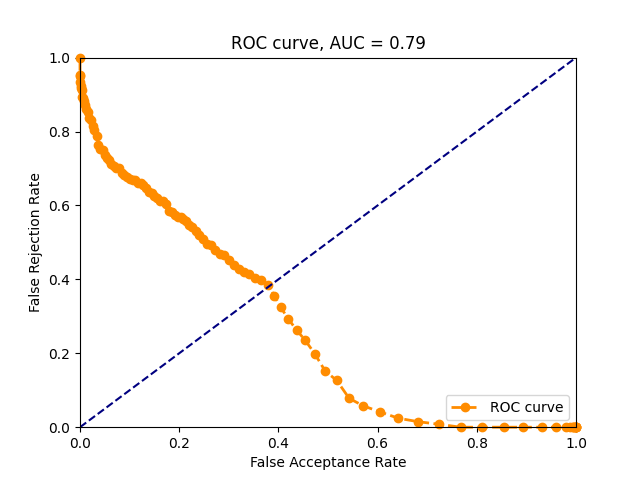
\includegraphics[width=.35\textwidth]{Manuscripts/src/figures/0.2_L_ROC.png}
                 \caption{Samples sequence with corresponding output values.}
                 \label{fig:ROC_fcn}
             \end{subfigure} 
                \caption{Converting time-series signal to the supervised data. For this example, window size is equal to 3. }
                \label{fig:ROC}
        \end{figure}
    \end{frame}

    \begin{frame}{Results}
        \begin{figure}[H]
            \centering
            \begin{minipage}[b]{1\textwidth}
                \includegraphics[width=\textwidth]{figures/0.2_L_ACC.png}
            \end{minipage}
            \caption{Resampling plot of the first dataset. The period of this dataset is 365 samples/cycle. }
            \label{fig:Ass1_D1_resample}
        \end{figure}
        \begin{columns}
            \begin{column}{0.5\textwidth}
                \begin{enumerate}
                    \item Sample size 20 participants
                    \item Duration 180 days
                    \item Minimum of 42 surveys per week
                \end{enumerate}
            \end{column}
            \begin{column}{0.5\textwidth}
                \begin{enumerate}
                    \item Sample size 20 participants
                    \item Duration 180 days
                    \item Minimum of 42 surveys per week
                \end{enumerate}
            \end{column}
        \end{columns}
    \end{frame}
    
    
    
    




\end{document}